\section{Multiples et diviseurs d'un nombre entier} 

% remarque : pour qu'un mot se retrouve dans le lexique : \MotDefinition{asymptote horizontale}{} 

\begin{aconnaitre}[Multiples et diviseurs]
\emph{12 $=$ 3 $\times$ 4}. On dit que :

\textcolor{C2}{\emph{12} est un multiple de \emph{3 (et de 4)}}

\textcolor{A1}{\emph{12} est divisible par \emph{3 (et par 4)}} ou \textcolor{J1}{\emph{3} est un diviseur de \emph{12}} ou \textcolor{H1}{\emph{3} divise \emph{12}}.
\end{aconnaitre}



%%%%%

\begin{methode*1}[Multiples, diviseurs]

\begin{exemple*1}
91 est-il un multiple de 7 ? 974 est-il divisible par 8 ? \\[1em]
\begin{minipage}[t]{0.46\linewidth}
$91 \div 7 = 13$ donc $91 = 7 \cdot 13$.

91 est donc un multiple de 7 (et de 13). On dit également que 91 est divisible par 7 (et par 13), que 7 est un diviseur de 91 (13 l'est aussi) ou que 7 divise 91 (13 divise aussi 91).
 \end{minipage} \hfill%
 \begin{minipage}[t]{0.46\linewidth}
 $974 : 8 = 121,75$.
 
121,75 n'est pas un entier, 974 n'est donc pas divisible par 8. On peut dire également que 8 n'est pas un diviseur de 974 et que 974 n'est pas un multiple de 8.
\end{minipage} \\

\end{exemple*1}

\exercice 
Établis la liste des diviseurs des entiers suivants : 60, 43 et 36.

\vspace{5em}


%\dotfill

%\dotfill

%\dotfill
%\correction

\exercice 
Détermine si 847 est un multiple de 7 :

%\dotfill

%\dotfill
%\correction

\end{methode*1}

%%%%%
  
\begin{aconnaitre}[Critères de divisibilité]
Un nombre entier est \textbf{\textcolor{A1}{divisible par 2}} si son chiffre des unités est pair (0, 2, 4, 6 ou 8) ;

Un nombre entier est \textbf{\textcolor{A1}{divisible par 3}} si la somme de ses chiffres est un multiple de 3 ;

Un nombre entier est \textbf{\textcolor{A1}{divisible par 6}} si il est divisible par 2 et par 3 ;

Un nombre entier est \textbf{\textcolor{A1}{divisible par 9}} si la somme de ses chiffres est un multiple de 9 ;

Un nombre entier est \textbf{\textcolor{A1}{divisible par 5}} si son chiffre des unités est 0 ou 5 ;

Un nombre entier est \textbf{\textcolor{A1}{divisible par 10}} si son chiffre des unités est 0 ;

Un nombre entier est \textbf{\textcolor{A1}{divisible par 25}} si ses deux derniers chiffres forment un nombre divisible par 25 (donc s'il se termine par 00, 25, 50 ou 75).
\end{aconnaitre}




\begin{methode*1}[Critères de divisibilité]

\begin{exemple*1}
750 est-il divisible par 2, par 3, par 6, par 5, par 9, par 10, par 25 ?
\begin{itemize}
 \item Le chiffre des unités de 750 est 0 donc 750 est divisible par 2, par 5 et par 10 ;
 \item La somme des chiffres de 750 est 12, divisible par 3 donc 750 est divisible par 3 mais pas par 9 ;
 \item 750 est divisible par 2 et 3 donc il est divisible par 6 ;
 \item Les deux  chiffre de 750 forment le nombre 50 donc 750 est divisible par 25.
 \end{itemize}
 \end{exemple*1}
 
 \begin{exemple*1}
Détermine des diviseurs de 23\,958 à l'aide des critères de divisibilité :
\begin{itemize}
 \item Le chiffre des unités de 23\,958 est 8 donc 23\,958 est divisible par 2 mais pas par 5 et ni par 10 ;
 \item La somme des chiffres de 23\,958 est $2 + 3 + 9 + 5 + 8$ soit 27. Comme 27 est divisible par 3 et par 9 donc 23\,958 est divisible par 3 et par 9 ;
 \item 2, 3 et 9 sont donc des diviseurs de 23\,958.
 \end{itemize}
 \end{exemple*1}

\begin{exemple*1}
Établis la liste de tous les diviseurs de 75.\\[1em]
Pour cela, on cherche tous les produits d'entiers positifs égaux à 75. \\[1em]
\begin{tabularx}{\textwidth}{c|X}
 $75 = \textcolor{J1}{1} \cdot \textcolor{A1}{75}$ &  Un nombre est toujours divisible par 1 et par lui-même. \\ 
 $75 = \textcolor{J1}{3} \cdot \textcolor{A1}{25}$ & Les critères de divisibilité permettent de dire que 75 est divisible par 3 et 5 mais qu'il n'est pas divisible par 9 et 10. \\
 $75 = \textcolor{J1}{5} \cdot \textcolor{A1}{15}$ & Les divisions par 4, 6, 7, 8, 11, 12, 13 et 14 ne donnant pas de quotients entiers, 75 n'est pas divisible par ces entiers.
 
Le diviseur suivant est 15 et on l'a déjà obtenu avec le produit $5 \cdot 15$ : on peut donc arrêter la recherche. \\
\end{tabularx} \\[1em]
Les diviseurs de 75 sont donc : \textcolor{J1}{1} ; \textcolor{J1}{3} ; \textcolor{J1}{5} ; \textcolor{A1}{15} ; \textcolor{A1}{25} et \textcolor{A1}{75}.
 \end{exemple*1}



\exercice  
Trouve toutes les possibilités pour le chiffre manquant $\#$, sachant que 3 et 2 divisent le nombre $2\,0\#4$ :

%\dotfill

%\dotfill

%\correction
 

 \end{methode*1}
 
 
%%%%%%%%%%%%%%%%%%%%%%%%%%%%%%%%%%%%%%%%%%%%%%%%%%%%%%%%%%%%%

\section{Puissances d'un nombre}

\begin{aconnaitre}
Pour gagner du temps et de la place, si on multiplie le nombre 4, 6 fois par lui même, au lieu d'écrire : $4 \times 4 \times 4 \times 4 \times 4 \times 4$, on utilise l'écriture des «puissances» et on écrit : $4^6$ qui se lit «4 puissance 6» ou «4 exposant 6».

De même on écrit $7^5$ pour écrire plus rapidement $7 \times 7 \times 7 \times 7 \times 7$. \\[1em]
En mathématiques, on dit que pour tout nombre $a$ non nul et tout nombre entier $n$ positif non nul : $a^n = \stackrel{n \text{ facteurs}}{\overbrace{a \cdot a \cdot a \cdot \ldots \cdot a}}$. On dit que $a$ est la base et $n$ est l'exposant. \\[1em]

$a^n$ se lit «$a$ exposant $n$» ou «$a$ puissance $n$».

\textbf{Cas particuliers} : 
\begin{itemize}
 \item Tout nombre à la puissance 1 est égal à lui même : 
 
 $3^1 = 3$, $21^1 = 21$ ;
 \item De plus, par convention, tout nombre non nul à la puissance 0 égal 1 : 
 
 $2^0 = 5^0 = 321^0 = 1$ ;
 \item Au lieu de dire «puissance 2», on dit «au carré». 
 
 Par exemple $5^2$ se lit «5 au carré».
 \end{itemize}
\end{aconnaitre}

\vspace{4em}

\begin{methode*1}[Utiliser la notation « puissance »]

\begin{exemple*1}
 : Les carrés des premiers entiers. \\[1em]
Il faut connaître les carrés des premiers nombres entiers : 

\begin{tabularx}{0.7\textwidth}{llllll}
$0^2 = 0$	& $1^2 = 1$ & $2^2 = 4$ & $3^2 = 9$ & $4^2 = 16$ & $5^2 = 25$ \\
$6^2 = 36$ & $7^2 = 49$ & $8^2 = 64$ & $9^2 = 81$ & $10^2 = 100$ & $11^2 = 121$ \\ 
$12^2 = 144$ & $13^2 = 169$ & & & & \\
 \end{tabularx} \\
 \end{exemple*1}

\begin{exemple*1}
Donne l'écriture décimale des nombres : $2^4$ et $2^3 \cdot 3^2$. \\[1em]
$2^4 =  2 \cdot 2 \cdot 2 \cdot 2 = 16$ ;

$2^3 \cdot 3^2 = 2 \cdot 2 \cdot 2 \cdot 3 \cdot 3 = 8 \cdot 9 = 72$.
 \end{exemple*1}

\exercice  
Donne l'écriture décimale des nombres : 

$A = 3^4$ ; $B = 3^2 \cdot 5^2$ ; $C = (5 \cdot 3)^2$.

\vspace{6em}

%\correction

 \end{methode*1}
 
 
 %%%%%%%%%%%%%%%%%%%%%%%%%%%%%%%%%%%%%%%%%%%%%%%%%%%%%%%%%%%%%

\newpage

\section{Nombres premiers et décomposition en produit de facteurs premiers}


\vspace{6em}

\begin{definition}
Un entier positif est un \MotDefinition{nombre premier}{} s'il admet exactement deux diviseurs distincts entiers et positifs (qui sont alors 1 et lui-même).
\end{definition}

\begin{remarque}
Cette définition exclut 1, qui n'a qu'un seul diviseur entier positif.
 \end{remarque}


\vspace{6em}


\begin{methode*1}[Nombres premiers]


 \begin{exemple*1}
 Détermine si 27 est un nombre premier : \\[1em]
 Pour cela on cherche s'il existe un diviseur de 27 différent de 1 et de 27.
 
27 n'est pas premier car 3 ou 9 sont des diviseurs de 27. \\[1em]
  \textcolor{A1}{Les nombres premiers inférieurs à 100 sont : 2, 3, 5, 7, 11, 13, 17, 19, 23, 29, 31, 37, 41, 43, 47, 53, 59, 61, 67, 71, 73, 79, 83, 89 et 97.}
  \end{exemple*1}

\exercice  

114 est-il un nombre premier ? Et 141 ?

 \end{methode*1}


\vspace{6em}


\begin{aconnaitre}
Tout nombre entier positif peut se décomposer de manière unique en un produit de facteurs premiers.
\end{aconnaitre}

\newpage

\begin{methode*1}[Décomposition en produits de facteurs premiers à l'aide d'un exemple]

\begin{exemple*1}
Donne la décomposition de 126 en produit de facteurs premiers.\\[1em]
Méthode : On cherche les nombres premiers qui divisent 126 (il est conseillé de chercher dans l'ordre croissant pour éviter d'en oublier). \\[1em]
\begin{tabularx}{\textwidth}{c|c|X}
 126 & \textcolor{A1}{2} & 126 est divisible par 2 : on fait la division qui a pour résultat 63 ; \\ 
 63 & \textcolor{A1}{3} & 63 n'est pas divisible par 2 mais est divisible par 3. Le résultat de la division est 21 ; \\
 21 & \textcolor{A1}{3} & 21 est encore divisible par 3. Le résultat de la division est 7 ; \\
7 & \textcolor{A1}{7} & 7 est un nombre premier : il est divisible par lui-même ; \\
1 & & Le dernier résultat obtenu dans la colonne de gauche est 1. On a trouvé tous les facteurs premiers de 126 : ils sont dans la colonne de droite. \\
\end{tabularx} \\[1em]
126 est égal au produit de tous les nombres qui sont dans la colonne de droite :
\begin{center} $126 = \textcolor{A1}{2} \cdot \textcolor{A1}{3} \cdot \textcolor{A1}{3} \cdot \textcolor{A1}{7} \textcolor{A1}{= 2 \cdot 3^2 \cdot 7}$ \end{center}
 \end{exemple*1}
 
\begin{remarque}
Si un nombre est divisible par 10, 100, 1000 \ldots, on peut gagner du temps en déterminant d'abord les facteurs premiers qui composent 10, 100, 1000 \ldots
\end{remarque}


\exercice  
Donne la décomposition en produit de facteurs premiers de 390 et 594.

\vspace{3em}
%\correction

 \end{methode*1}
 
 %%%%%%%%%%%%%%%%%%%%%%%%%%%%%%%%%%%%%%%%%%%%%%%%%%%%%%%%%%%%%
 
 \newpage
 
 \section{Plus Grand Diviseur Commun (PGCD)}
 
 \begin{definition}
Étant donné deux nombres $a$ et $b$, on peut chercher le plus grand nombre qui divise à la fois $a$ et $b$. Ce nombre est leur Plus Grand Diviseur Commun que l'on appelle \MotDefinition{PGDC}{}.
\begin{itemize}
 \item Si le PGDC de deux entiers positifs est 1, on dit que ces deux entiers sont \textbf{premiers entre eux} (attention, à ne pas confondre «deux nombres premiers entre eux» et «un nombre premier»).
 \item Si un nombre divise un autre nombre, par exemple 12 divise 48, alors PGDC $(12 ; 48) = 12$.
 \end{itemize}
\end{definition}
 
 \vspace{1em}
 
 Pour trouver le PGDC de deux nombres entiers positifs, on peut utiliser deux méthodes (il en existe d'autres qui ne sont pas au programme) : \\[1em]


 \begin{methode*1}[Déterminer le PGDC avec la liste de tous les diviseurs]

\textcolor{H1}{\textbf{Méthode 1}} : On cherche tous les diviseurs de chacun des deux nombres en on prend le plus grand diviseur qu'ils ont en commun.

\begin{exemple*1}
Déterminer le PGDC de 12 et 18 en trouvant tous les diviseurs de 12 et tous ceux de 18 : \\[1em]
\begin{tabularx}{\textwidth}{l|X}
 $12 = \textcolor{J1}{1} \cdot \textcolor{A1}{12}$ & Un nombre est toujours divisible par 1 et par lui-même donc 12 est divisible par 1 et par 12 ; \\ 
 $\textcolor{A1}{12 }= \textcolor{A1}{2} \cdot \textcolor{A1}{6}$ & Les critères de divisibilité permettent de dire que 12 est divisible par 2 et 3 ; \\
 $\textcolor{A1}{12} = \textcolor{A1}{4} \cdot \textcolor{A1}{3}$ & Les diviseurs de 12 sont donc : 1 ; 2 ; 3 ; 4 ; 6 ; 12 ; \\
 $18 = \textcolor{J1}{1} \cdot \textcolor{A1}{18}$ & Un nombre est toujours divisible par 1 et par lui-même donc 18 est divisible par 1 et par 18 ; \\ 
 $\textcolor{A1}{18} = \textcolor{A1}{2} \cdot \textcolor{A1}{9}$ & Les critères de divisibilité permettent de dire que 18 est divisible par 2 et 3 ; \\
 $\textcolor{A1}{18} = \textcolor{A1}{3} \cdot \textcolor{A1}{6}$ & Les diviseurs de 18 sont donc : 1 ; 2 ; 3 ; 6 ; 18. \\
\end{tabularx} \\[1em]
Conclusion : avec la liste des diviseurs de 12 et des diviseurs de 18, on voit que le plus grand diviseur commun à 12 et 18 est 6. \\[-2em]
 \end{exemple*1}
 
\vspace{1em}

\textcolor{H1}{\textbf{Remarque}} :L'avantage de cette méthode est qu'il est très facile de trouver le PGDC quand on a la liste de tous les diviseurs. L'inconvénient, c'est qu'il est parfois très long de trouver tous les diviseurs des deux nombres.


 \exercice  
Déterminer le PGCD de 45 et 75. la liste des diviseurs de 75 se trouve plus haut dans ce cours.

\vspace{2em}

%\correction

\exercice  
Déterminer le PGCD de 35 et 42.

%\correction

%\exercice  
%Quel est le plus grand nombre entier divisant à la fois 84 et 180?


%\correction

 \end{methode*1}




\newpage




\begin{methode*1}[Déterminer le PGDC avec la décomposition en produits de facteurs premiers]

\textcolor{H1}{\textbf{Méthode 2}} : On décompose les deux nombres en produit de facteurs premiers. On trouve ensuite le PGDC en faisant le produit de tous les facteurs qui sont en commun dans la décomposition des deux nombres.

\begin{exemple*1}
Détermine le PGDC de 30 et 45 et décomposant 30 et 45 en produit de facteurs premiers : \\[1em]
\begin{minipage}[t]{0.36\textwidth}
 \begin{tabularx}{0.4\textwidth}{X|X}
 30 & 2 \\ 
 15 & 3 \\
 5 & 5 \\
 1 & \\ 
 \end{tabularx} \\[1em]
$30 = 2 \times 3 \times 5$ 
\end{minipage} \hfill%
\begin{minipage}[t]{0.56\textwidth}
 \begin{tabularx}{0.3\textwidth}{X|X}
 45 & 3 \\ 
 15 & 3 \\
 5 & 5 \\
 1 & \\ 
 \end{tabularx} \\[1em]
$45 = 3 \times 3 \times 5$

 \end{minipage} \\

Le PGDC de 30 et 45 est donc égal au produit des facteurs premiers que l'on trouve dans les deux décompositions, soit 3 et 5 (attention, 3 n’apparaît qu'une seule fois dans la décomposition de 30 donc on ne le prend qu'une seule fois dans le calcul du PGDC).
On note PGDC $(30 ; 45) = 3 \times 5 = 15$. \\[-2em]
 \end{exemple*1}

 \vspace{1em}

\textcolor{H1}{\textbf{Remarque}} :
L'avantage de cette méthode est qu'elle est plus rapide mais il ne faut pas se tromper dans le choix des facteurs communs aux deux nombres (surtout quand certains facteurs sont écrits avec des puissances).


\exercice  
Déterminer le PGCD de 45 et 75 (la liste des diviseurs de 75 se trouve plus haut dans ce cours…).

\vspace{3em}
%\correction

\exercice  
Déterminer le PGCD de 35 et 42.

\vspace{5em}
%\correction

\exercice  
Quel est le plus grand nombre entier divisant à la fois 84 et 180?

\vspace{3em}
%\correction

 \end{methode*1}
 %%%%%%%%%%%%%%%%%%%%%%%%%%%%%%%%%%%%%%%%%%%%%%%%%%%%%%%%%%%%%
 \newpage
\begin{activite}[Problème: Portefeuille oublié!]
Eddy et Dimitri, tous deux chauffeurs aux TPG, sont amis de puis de nombreuses années.\\
À 14h47, Eddy s’aperçoit qu’il a oublié son portefeuille dans le bus qu’il conduisait ce matin. Il appelle alors Dimitri qui lui promet de le lui rendre dès qu’ils se croiseront de nouveau à un arrêt.\\
A quel moment et où Dimitri pourra-t-il rendre son portefeuille à Eddy?
\newline
Pour répondre à cette question, vous trouverez ci-joint: un plan des bus de la ville de Genève et les feuilles de services des deux chauffeurs.\\
Si vous avez besoin de documents supplémentaires, n'hésitez pas à demander à votre professeur; il pourra sans doute vous aider!!

\begin{center}
    \includegraphics[width=14cm]{NbsEntiers_Multiples_Diviseurs/figures/planTPG.eps}\\
\end{center}

\begin{minipage}[t]{0.50\linewidth}
\begin{center}
    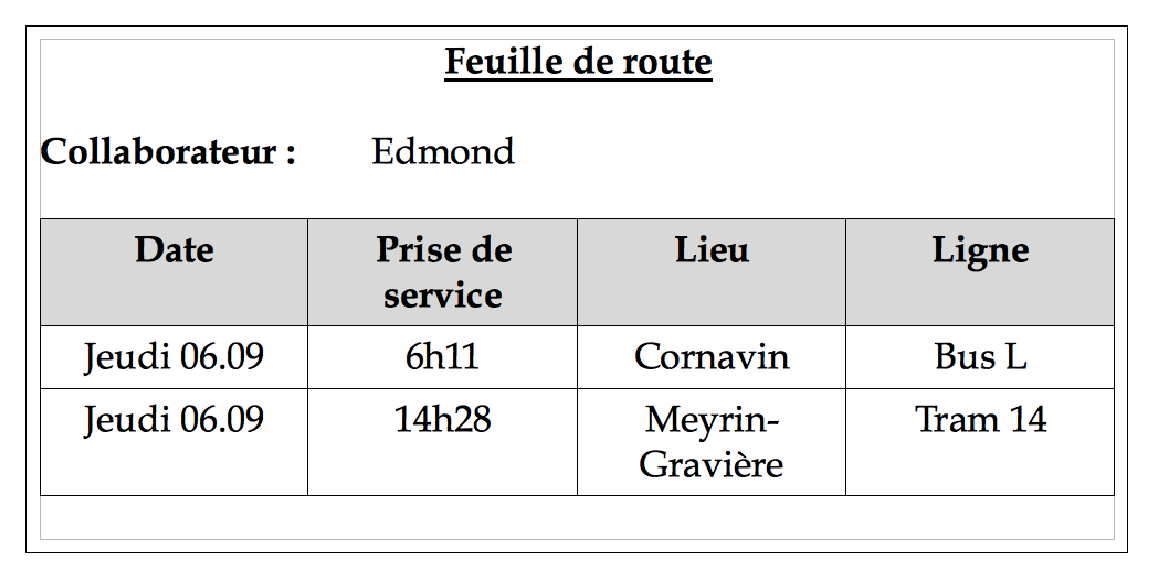
\includegraphics[width=7cm]{NbsEntiers_Multiples_Diviseurs/figures/Eddy.eps}
\end{center}
\end{minipage}
\begin{minipage}[t]{0.50\linewidth}
\begin{center}
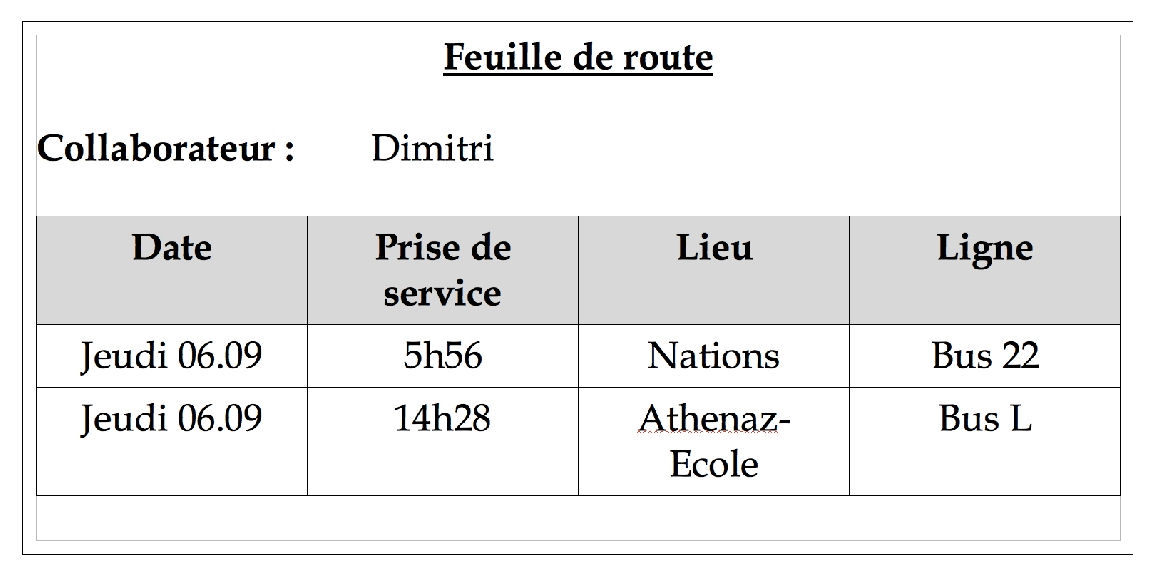
\includegraphics[width=7cm]{NbsEntiers_Multiples_Diviseurs/figures/Dimitri.eps}
\end{center}
\end{minipage}

\prof{Les élèves auront besoin de connaître les temps de trajet des lignes 14 et L. Voici ce que l'on trouve à ce sujet sur le site des TPG:\\
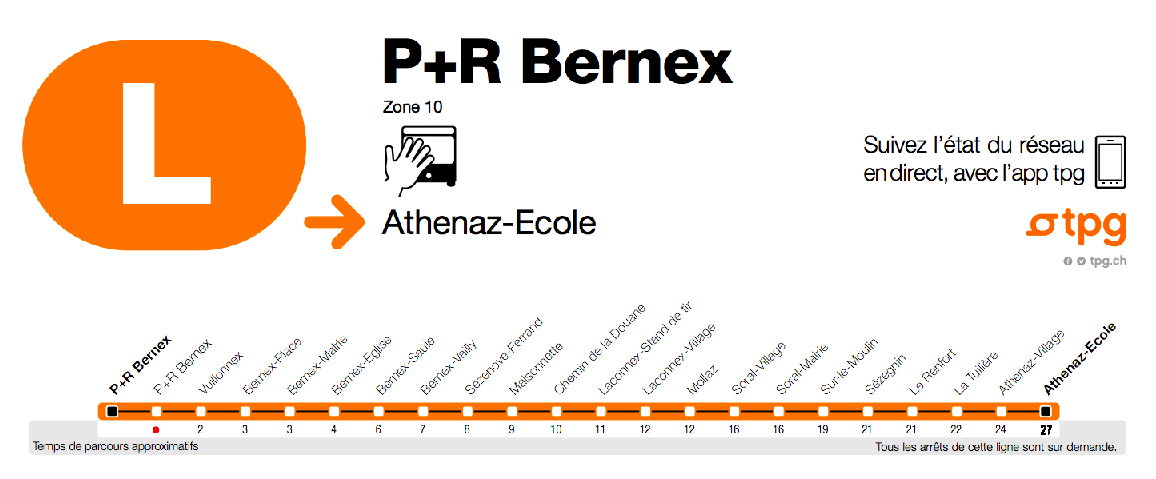
\includegraphics[width=14cm]{NbsEntiers_Multiples_Diviseurs/figures/ligneL.eps}\\
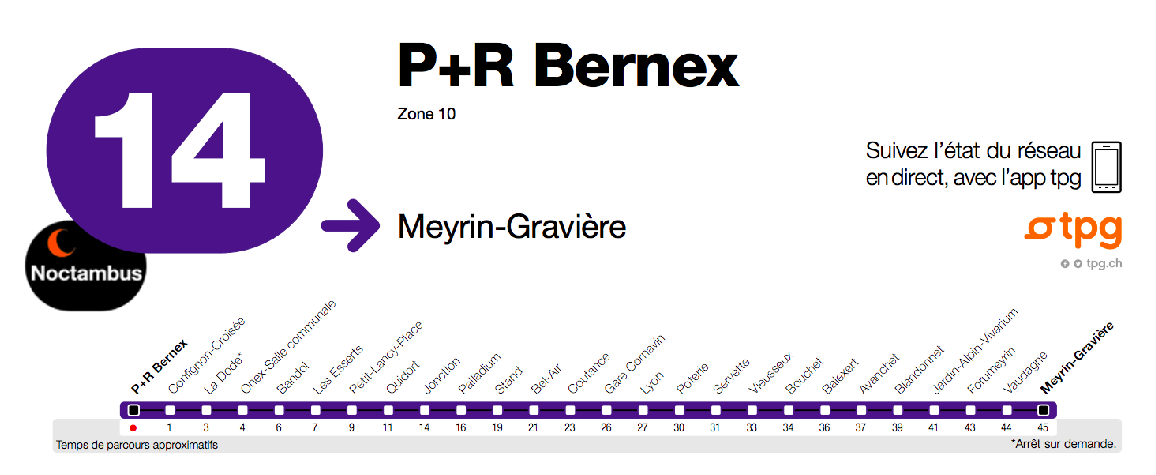
\includegraphics[width=14cm]{NbsEntiers_Multiples_Diviseurs/figures/ligne14.eps}\\
Je propose d'attendre que les élèves demandent les horaires de ces lignes pour leur fournir ces informations.
}

\end{activite}

 %%%%%%%%%%%%%%%%%%%%%%%%%%%%%%%%%%%%%%%%%%%%%%%%%%%%%%%%%%%%%
  %%%%%%%%%%%%%%%%%%%%%%%%%%%%%%%%%%%%%%%%%%%%%%%%%%%%%%%%%%%%%
 
 \newpage
 
 \section{Plus Petit Multiple Commun (PPCM)}
 
\begin{definition}
Le \MotDefinition{PPMC de deux entiers positifs}{} est leur Plus Petit Multiple Commun.
\end{definition}

 \begin{remarque}
Le PPMC de deux nombres n'est jamais plus grand que le produit des deux nombres.

Si un nombre est le multiple d'un autre : par exemple 15 est multiple de 3, alors 15 est le PPMC de 15 et 3.
 \end{remarque}
 
 \vspace{2em}
 
 Pour trouver le PPMC de deux nombres entiers positifs, on peut utiliser deux méthodes :  \\[1em]


 %\vspace{2em}

\begin{methode*1}[Déterminer le PPMC avec les premiers multiples ]
 
\textcolor{H1}{\textbf{PPMC, 1\up{ère} méthode}} : On cherche les premiers multiples de chacun des deux nombres en on prend le plus petit qu'ils ont en commun.

\begin{exemple*1}
Déterminer le PPMC de 12 et 18 en écrivant les premiers multiples de 12 et de 18 : \\[1em]
 \begin{tabularx}{\textwidth}{l|X}
 \textcolor{A1}{12 $\times$ 1 $=$ 12} & Les premiers multiples de 12 sont donc :  \\ 
 \textcolor{A1}{12 $\times$ 2 $=$ 24} &  12 ; 24 ; 36 ; 48.\\
 \textcolor{A1}{12 $\times$ 3 $=$ \textbf{36}} &  \\
 \textcolor{A1}{12 $\times$ 4 $=$ 48} &  \\ 
 \textcolor{A1}{18 $\times$ 1 $=$ 18} &  \\
 \textcolor{A1}{18 $\times$ 2 $=$ \textbf{36}} &  \\
 \textcolor{A1}{18 $\times$ 3 $=$ 54} & Les premiers multiples de 18 sont donc : 18  ; 36 ; 54. \\
\end{tabularx} \\[1em]
Conclusion : avec la liste des premiers multiples de 12 et ceux de 18, on voit que le plus petit multiple commun à 12 et 18 est 36. \\%[-2em]
 \end{exemple*1}

\vspace{1em}

\textcolor{H1}{\textbf{Remarque}} : L'avantage de cette méthode est qu'il est très facile de trouver le PPMC quand on a la liste des premiers multiples. Elle est aussi souvent plus rapide avec des petits nombres. L'inconvénient, c'est qu'il est parfois très long de trouver un premier multiple commun aux deux nombres quand les deux nombres sont grands.
 
 \exercice
Calculer les 5 premiers multiples de 6 et 10 et déterminer leur PPMC.

\vspace{3em}
 

%\correction

 \exercice
Décomposer 120 et 252 en produit de facteurs premiers puis déterminer leur PPMC.
 
%\vspace{3em}
%\correction

 \end{methode*1}
 
 \newpage
 
 
 \vspace{2em}

 
\begin{methode*1}[Déterminer le PPMC avec la décomposition en produits de facteurs premiers]

\textcolor{H1}{\textbf{PPMC, 2\up{e} méthode}} : On décompose les deux nombres en produit de facteurs premiers. On trouve ensuite le PPMC en faisant le produit de tous les facteurs qui apparaissent dans l'une {\textbf ou} l'autre décomposition. Si le facteur premier apparaît dans les deux décompositions, on le prend avec la plus grande puissance qui apparaît.

\begin{exemple*1}
Déterminer le PPMC de 30 et 45 et décomposant 30 et 45 en produit de facteurs premiers : \\[1em]
\begin{minipage}[t]{0.36\textwidth}
 \begin{tabularx}{0.4\textwidth}{X|X}
 30 & 2 \\ 
 15 & 3 \\
 5 & 5 \\
 1 & \\ 
 \end{tabularx} \\[1em]
\end{minipage} \hfill%
\begin{minipage}[t]{0.56\textwidth}
 \begin{tabularx}{0.3\textwidth}{X|X}
 45 & 3 \\ 
 15 & 3 \\
 5 & 5 \\
 1 & \\ 
 \end{tabularx} \\[1em]
 \end{minipage} \\
Les facteurs qui apparaissent sont 2 ; 3 et 5. 3 apparaît dans les deux décompositions mais avec une puissance 1 dans la décomposition de 30 et avec une puissance 2 dans celle de 45. Donc on prend le $3^2$ pour le calcul du PPMC.

Le PPMC de 30 et 45 est donc égal à $2 \times 32 \times 5 = 90$.

On note PPMC $(30 ; 45) = 90$ ou PPMC $(45 ; 30) = 90$. \\[-2em]
 \end{exemple*1}
 
\vspace{2em}

\textcolor{H1}{\textbf{Remarque}} :
L'avantage de cette méthode est qu'elle est plus rapide avec les grands nombres mais il ne faut pas se tromper dans le choix des facteurs communs aux deux nombres (surtout quand certains facteurs sont écrits avec des puissances).

 

 \exercice
Calculer les 5 premiers multiples de 6 et 10 et déterminer leur PPMC.
 
\vspace{5em}

%\correction

 \exercice
Décomposer 120 et 252 en produit de facteurs premiers puis déterminer leur PPMC.

\vspace{5em}

%\correction

 \end{methode*1}
 
